% Set up the standalone document clas
\documentclass{standalone}

% Input the preamble (<3)
% Preamble document

% Import tikz package
\usepackage{tikz}

% Import tikz libraries
\usetikzlibrary{shapes, arrows}
\usetikzlibrary{positioning, calc}

%----------- Create a fancy summing block
\tikzset{add/.style n args={4}{
		minimum width=6mm,
		path picture={
			\draw[black] 
			(path picture bounding box.south east) -- (path picture bounding box.north west)
			(path picture bounding box.south west) -- (path picture bounding box.north east);
			\node at ($(path picture bounding box.south)+(0,0.13)$)     {\tiny #1};
			\node at ($(path picture bounding box.west)+(0.13,0)$)      {\tiny #2};
			\node at ($(path picture bounding box.north)+(0,-0.13)$)    {\tiny #3};
			\node at ($(path picture bounding box.east)+(-0.13,0)$)     {\tiny #4};
		}
	}
}

%----------- Block style 1
\tikzstyle{block1} = [draw, fill=blue!20, rectangle, 
minimum height=3em, minimum width=6em, node distance=2.5cm]

%----------- Block style 2
\tikzstyle{block2} = [draw, fill=blue!20, rectangle, 
minimum height=3em, minimum width=3em, node distance=2.5cm]

%----------- Sum style
\tikzstyle{sum} = [draw, fill=blue!20, circle, node distance=2cm]

%----------- Input style
\tikzstyle{input} = [coordinate, node distance=4cm]

%----------- Output style
\tikzstyle{output} = [coordinate, node distance=4cm]

%----------- Pin style
\tikzstyle{pinstyle} = [pin edge={to-,thin,black}]

\usepackage{amsmath}

% Additional styles
\tikzstyle{blockn} = [rectangle, draw, text width=4em, text centered, rounded corners, minimum height=4em]
    
\tikzstyle{line} = [draw, -latex]

\tikzset{
    block/.style={
        draw,
        rectangle split,
        rectangle split parts=2,
        text centered,
        text width=8em,
        rounded corners,
        minimum height=4em
        }
}

\begin{document}
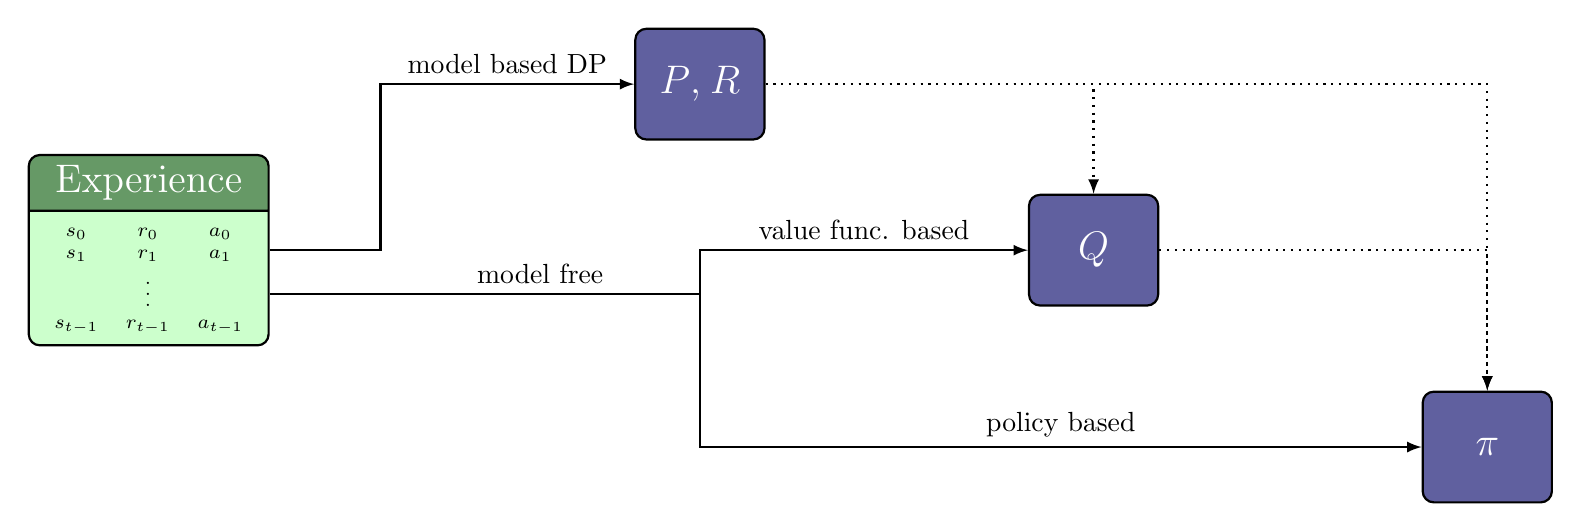
\begin{tikzpicture}[node distance = 6em, auto, thick]
    
	% Environment node
	\node [block, rectangle split empty part height=1cm, rectangle split part fill={green!20!gray,white!80!green}] (Environment) {\Large\textcolor{white}{Experience} \nodepart{second} \scriptsize $\begin{matrix}
	  		s_0 	& r_0 	  	& a_0  \\
	  		s_1 	& r_1 	  	& a_1  \\
	  				& \vdots	&	   \\
	  		s_{t-1} & r_{t-1} 	& a_{t-1}
	\end{matrix}$};
	
	\node [coordinate, right of=Environment, node distance=7cm] (c1) {};
	
	\node [blockn, above of=c1, fill=blue!25!gray, text=white] (dynamic) {\Large $P$, $R$};
	
	\node [blockn, right of=c1, node distance=5cm, fill=blue!25!gray, text=white] (value) {\Large $Q$};
	
	\node [coordinate, right of=value, node distance=5cm] (c2) {};
	
	\node [blockn, below of=c2, node distance=2.5cm, fill=blue!25!gray, text=white] (policy) {\Large $\pi$};
	
	\path [line] (Environment.0) --++ (4em,0em) |- node [near end]{model based DP} (dynamic.180);
	\path [line] (Environment.-20) --++ (4em,0em) -| node [near start] {model free} (c1) -- node {value func. based} (value.180);
	\path [line] (c1) |- node [near end] {policy based} (policy);
	
	\path [line, dotted] (dynamic.0) -| (value.90);
	\path [line, dotted] (value.0) -| (policy.90);
	\path [line, dotted] (dynamic.0) -| (policy.90);
		
\end{tikzpicture}
\end{document}